%!TeX root=../pridetop.tex
\chapter[Chapter \thechapter]{}
	
	
\begin{figure}[t!]
\centering
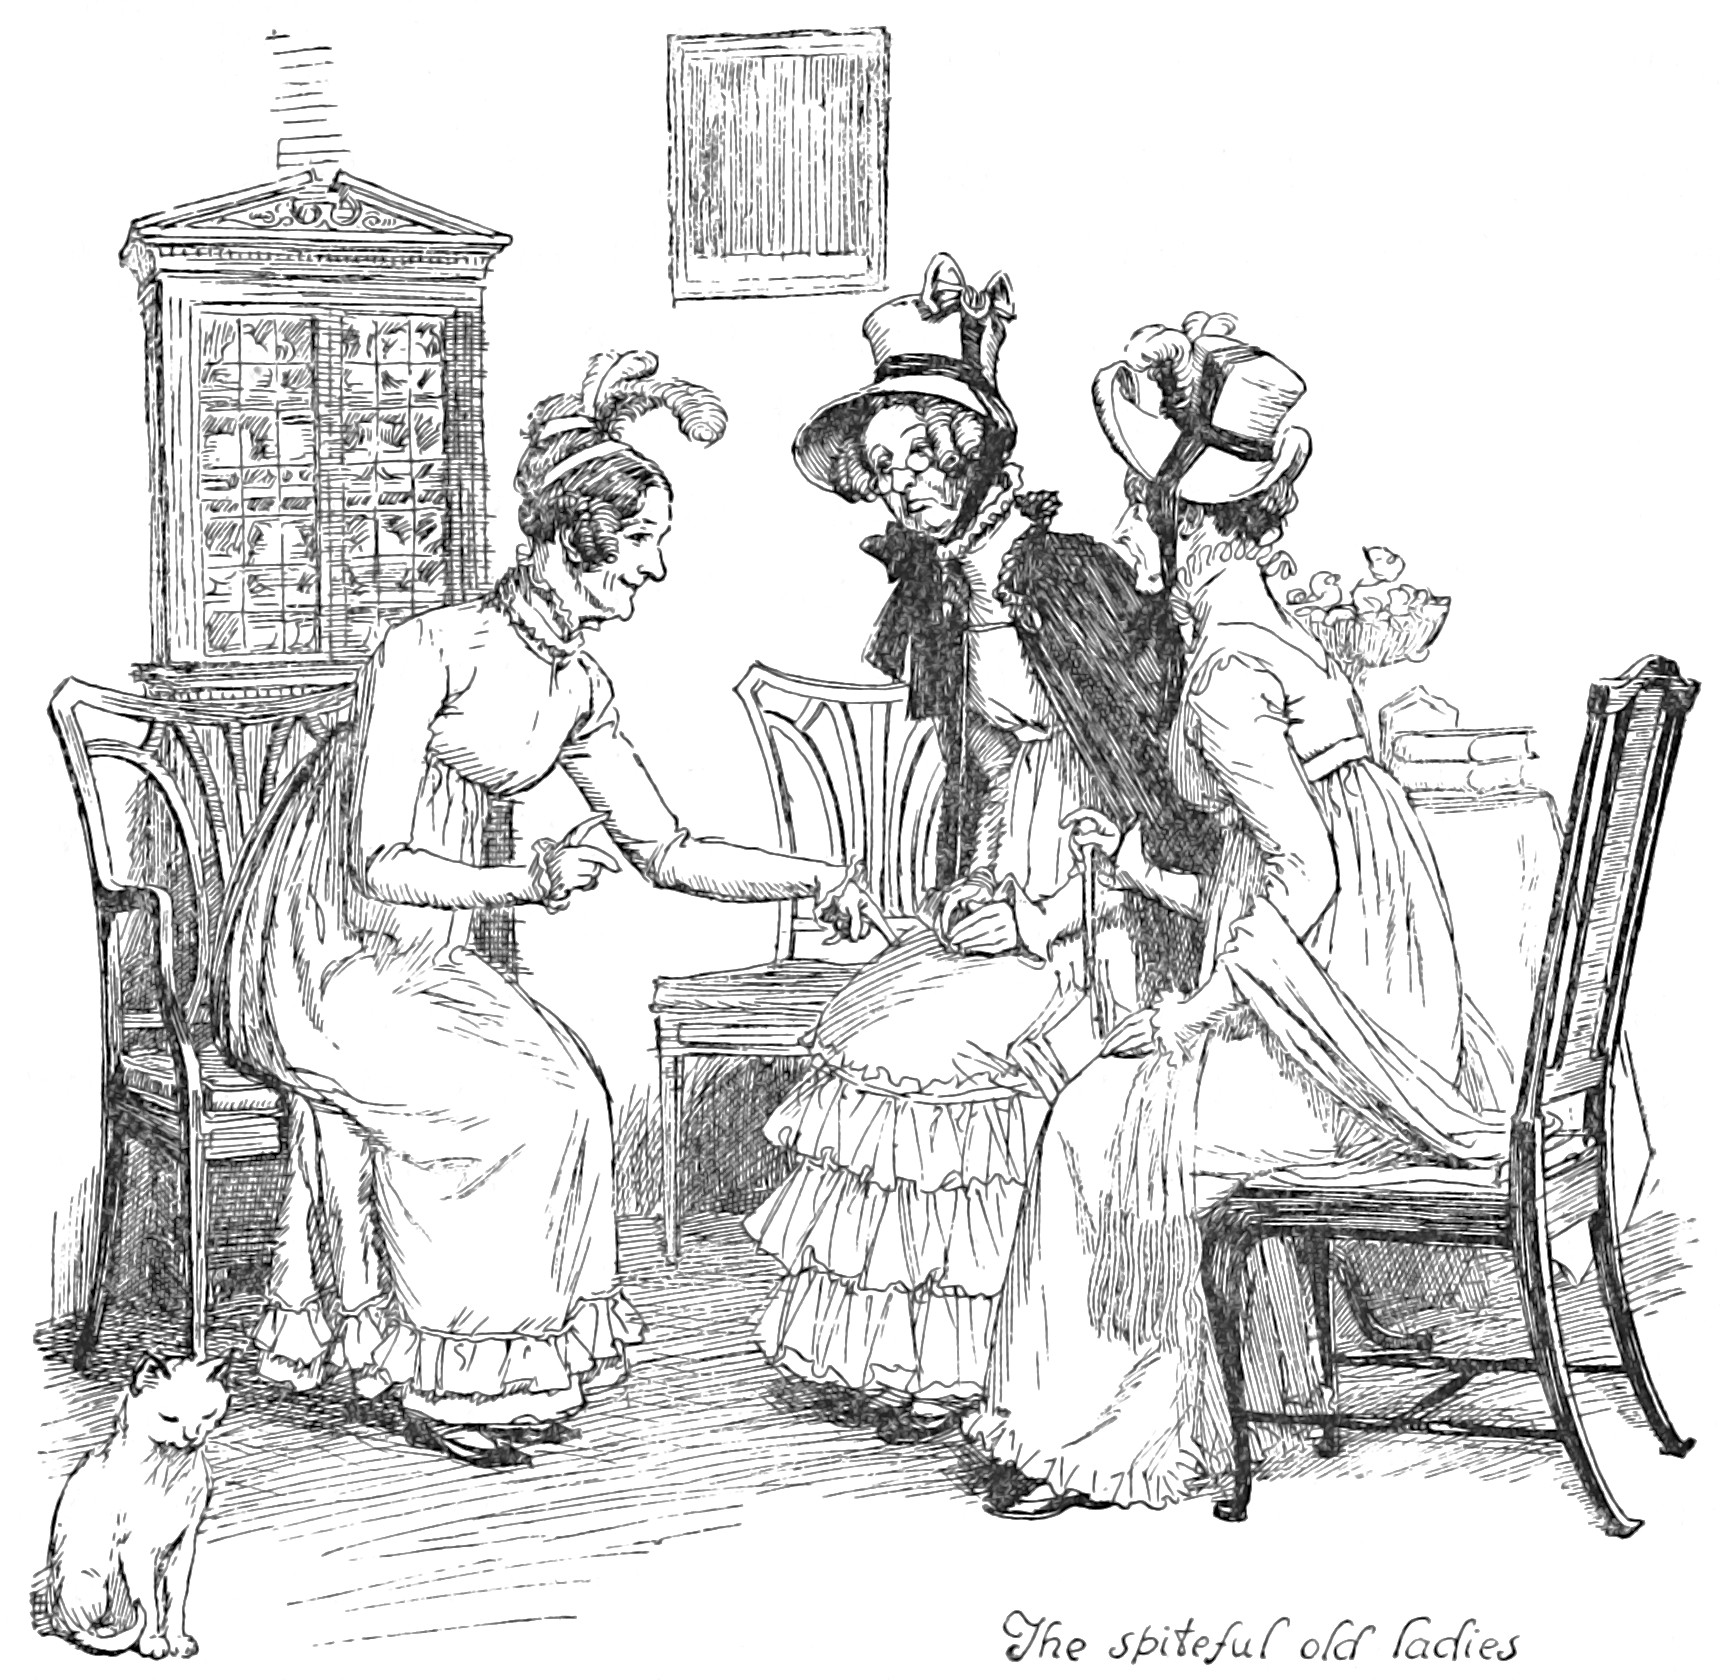
\includegraphics[width=.9\linewidth]{50top}
\captionlistentry{The spiteful old ladies}
\end{figure}


\lettrine[lines=6,image=true]{initials/chap50m}{r} Bennet had very often wished, before this period of his life, that, instead of spending his whole income, he had laid by an annual sum, for the better provision of his children, and of his wife, if she survived him. He now wished it more than ever. Had he done his duty in that respect, Lydia need not have been indebted to her uncle for whatever of honour or credit could now be purchased for her. The satisfaction of prevailing on one of the most worthless young men in Great Britain to be her husband might then have rested in its proper place.

He was seriously concerned that a cause of so little advantage to anyone should be forwarded at the sole expense of his brother-in-law; and he was determined, if possible, to find out the extent of his assistance, and to discharge the obligation as soon as he could.

When first Mr Bennet had married, economy was held to be perfectly useless; for, of course, they were to have a son. This son was to join in cutting off the entail, as soon as he should be of age, and the widow and younger children would by that means be provided for. Five daughters successively entered the world, but yet the son was to come; and Mrs Bennet, for many years after Lydia's birth, had been certain that he would. This event had at last been despaired of, but it was then too late to be saving. Mrs Bennet had no turn for economy; and her husband's love of independence had alone prevented their exceeding their income.

Five thousand pounds was settled by marriage articles on Mrs Bennet and the children. But in what proportions it should be divided amongst the latter depended on the will of the parents. This was one point, with regard to Lydia at least, which was now to be settled, and Mr Bennet could have no hesitation in acceding to the proposal before him. In terms of grateful acknowledgment for the kindness of his brother, though expressed most concisely, he then delivered on paper his perfect approbation of all that was done, and his willingness to fulfil the engagements that had been made for him. He had never before supposed that, could Wickham be prevailed on to marry his daughter, it would be done with so little inconvenience to himself as by the present arrangement. He would scarcely be ten pounds a year the loser, by the hundred that was to be paid them; for, what with her board and pocket allowance, and the continual presents in money which passed to her through her mother's hands, Lydia's expenses had been very little within that sum.

That it would be done with such trifling exertion on his side, too, was another very welcome surprise; for his chief wish at present was to have as little trouble in the business as possible. When the first transports of rage which had produced his activity in seeking her were over, he naturally returned to all his former indolence. His letter was soon despatched; for though dilatory in undertaking business, he was quick in its execution. He begged to know further particulars of what he was indebted to his brother; but was too angry with Lydia to send any message to her.

The good news quickly spread through the house; and with proportionate speed through the neighbourhood. It was borne in the latter with decent philosophy. To be sure, it would have been more for the advantage of conversation, had Miss Lydia Bennet come upon the town; or, as the happiest alternative, been secluded from the world in some distant farm-house. But there was much to be talked of, in marrying her; and the good-natured wishes for her well-doing, which had proceeded before from all the spiteful old ladies in Meryton, lost but little of their spirit in this change of circumstances, because with such a husband her misery was considered certain.

It was a fortnight since Mrs Bennet had been down stairs, but on this happy day she again took her seat at the head of her table, and in spirits oppressively high. No sentiment of shame gave a damp to her triumph. The marriage of a daughter, which had been the first object of her wishes since Jane was sixteen, was now on the point of accomplishment, and her thoughts and her words ran wholly on those attendants of elegant nuptials, fine muslins, new carriages, and servants. She was busily searching through the neighbourhood for a proper situation for her daughter; and, without knowing or considering what their income might be, rejected many as deficient in size and importance.

»Haye Park might do,« said she, »if the Gouldings would quit it, or the great house at Stoke, if the drawing-room were larger; but Ashworth is too far off. I could not bear to have her ten miles from me; and as for Purvis Lodge, the attics are dreadful.«

Her husband allowed her to talk on without interruption while the servants remained. But when they had withdrawn, he said to her, »Mrs Bennet, before you take any, or all of these houses, for your son and daughter, let us come to a right understanding. Into \textit{one} house in this neighbourhood they shall never have admittance. I will not encourage the imprudence of either, by receiving them at Longbourn.«

A long dispute followed this declaration; but Mr Bennet was firm: it soon led to another; and Mrs Bennet found, with amazement and horror, that her husband would not advance a guinea to buy clothes for his daughter. He protested that she should receive from him no mark of affection whatever on the occasion. Mrs Bennet could hardly comprehend it. That his anger could be carried to such a point of inconceivable resentment as to refuse his daughter a privilege, without which her marriage would scarcely seem valid, exceeded all that she could believe possible. She was more alive to the disgrace, which her want of new clothes must reflect on her daughter's nuptials, than to any sense of shame at her eloping and living with Wickham a fortnight before they took place.

Elizabeth was now most heartily sorry that she had, from the distress of the moment, been led to make Mr Darcy acquainted with their fears for her sister; for since her marriage would so shortly give the proper termination to the elopement, they might hope to conceal its unfavourable beginning from all those who were not immediately on the spot.

She had no fear of its spreading farther, through his means. There were few people on whose secrecy she would have more confidently depended; but at the same time there was no one whose knowledge of a sister's frailty would have mortified her so much. Not, however, from any fear of disadvantage from it individually to herself; for at any rate there seemed a gulf impassable between them. Had Lydia's marriage been concluded on the most honourable terms, it was not to be supposed that Mr Darcy would connect himself with a family, where to every other objection would now be added an alliance and relationship of the nearest kind with the man whom he so justly scorned.

From such a connection she could not wonder that he should shrink. The wish of procuring her regard, which she had assured herself of his feeling in Derbyshire, could not in rational expectation survive such a blow as this. She was humbled, she was grieved; she repented, though she hardly knew of what. She became jealous of his esteem, when she could no longer hope to be benefited by it. She wanted to hear of him, when there seemed the least chance of gaining intelligence. She was convinced that she could have been happy with him, when it was no longer likely they should meet.

What a triumph for him, as she often thought, could he know that the proposals which she had proudly spurned only four months ago would now have been gladly and gratefully received! He was as generous, she doubted not, as the most generous of his sex. But while he was mortal, there must be a triumph.

She began now to comprehend that he was exactly the man who, in disposition and talents, would most suit her. His understanding and temper, though unlike her own, would have answered all her wishes. It was an union that must have been to the advantage of both: by her ease and liveliness, his mind might have been softened, his manners improved; and from his judgment, information, and knowledge of the world, she must have received benefit of greater importance.

But no such happy marriage could now teach the admiring multitude what connubial felicity really was. An union of a different tendency, and precluding the possibility of the other, was soon to be formed in their family.

How Wickham and Lydia were to be supported in tolerable independence she could not imagine. But how little of permanent happiness could belong to a couple who were only brought together because their passions were stronger than their virtue, she could easily conjecture.

Mr Gardiner soon wrote again to his brother. To Mr Bennet's acknowledgments he briefly replied, with assurances of his eagerness to promote the welfare of any of his family; and concluded with entreaties that the subject might never be mentioned to him again. The principal purport of his letter was to inform them, that Mr Wickham had resolved on quitting the militia.


\begin{quotation}

\noindent It was greatly my wish that he should do so,

\end{quotation}


 he added, 

 
 \begin{quotation}
 \noindent as soon as his marriage was fixed on. And I think you will agree with me, in considering a removal from that corps as highly advisable, both on his account and my niece's. It is Mr Wickham's intention to go into the Regulars; and, among his former friends, there are still some who are able and willing to assist him in the army. He has the promise of an ensigncy in General—'s regiment, now quartered in the north. It is an advantage to have it so far from this part of the kingdom. He promises fairly; and I hope among different people, where they may each have a character to preserve, they will both be more prudent. I have written to Colonel Forster, to inform him of our present arrangements, and to request that he will satisfy the various creditors of Mr Wickham in and near Brighton with assurances of speedy payment, for which I have pledged myself. And will you give yourself the trouble of carrying similar assurances to his creditors in Meryton, of whom I shall subjoin a list, according to his information? He has given in all his debts; I hope at least he has not deceived us. Haggerston has our directions, and all will be completed in a week. They will then join his regiment, unless they are first invited to Longbourn; and I understand from Mrs Gardiner that my niece is very desirous of seeing you all before she leaves the south. She is well, and begs to be dutifully remembered to you and her mother.

\begin{flushright}
Yours, etc.\\
\textsc{E. Gardiner.}
\end{flushright}
\end{quotation}


Mr Bennet and his daughters saw all the advantages of Wickham's removal from the ——shire, as clearly as Mr Gardiner could do. But Mrs Bennet was not so well pleased with it. Lydia's being settled in the north, just when she had expected most pleasure and pride in her company, for she had by no means given up her plan of their residing in Hertfordshire, was a severe disappointment; and, besides, it was such a pity that Lydia should be taken from a regiment where she was acquainted with everybody, and had so many favourites.

»She is so fond of Mrs Forster,« said she, »it will be quite shocking to send her away! And there are several of the young men, too, that she likes very much. The officers may not be so pleasant in General—'s regiment.«

His daughter's request, for such it might be considered, of being admitted into her family again, before she set off for the north, received at first an absolute negative. But Jane and Elizabeth, who agreed in wishing, for the sake of their sister's feelings and consequence, that she should be noticed on her marriage by her parents, urged him so earnestly, yet so rationally and so mildly, to receive her and her husband at Longbourn, as soon as they were married, that he was prevailed on to think as they thought, and act as they wished. And their mother had the satisfaction of knowing, that she should be able to show her married daughter in the neighbourhood, before she was banished to the north. When Mr Bennet wrote again to his brother, therefore, he sent his permission for them to come; and it was settled, that, as soon as the ceremony was over, they should proceed to Longbourn. Elizabeth was surprised, however, that Wickham should consent to such a scheme; and, had she consulted only her own inclination, any meeting with him would have been the last object of her wishes.

